% !TeX root = ../main.tex
% 修改稿迁移版：自动编号，原文数据与待核事项保留。
\chapter{项目简介}
\section{命题内容}\label{sec:2.1}
人工智能正在从提供信息和辅助决策，向参与实际业务执行发展。代码修复、功能开发、数据分析等场景，不仅需要模型给出答案，还需要智能体调用工具、执行操作并完成任务。Gartner 于 2025 年发布预测，到 2026 年底，40\% 的企业应用将集成面向特定任务的智能体，而发布预测时这一比例不足 5\%。智能体应用范围的扩大，也将带动对配套运行环境和基础服务的需求。

尽管应用需求持续增长，但智能体从技术验证走向规模化落地，仍面临不少现实约束。Gartner 指出，部署成本上升、商业价值不明确以及风险控制不足，是智能体项目推进过程中面临的重要障碍。从企业实际使用角度看，智能体的价值不仅取决于单次任务能否完成，还取决于能否同时服务多个用户、持续稳定运行，以及投入与产出是否匹配。因此，支撑智能体运行的基础软件，需要在功能、安全、效率和成本之间形成适合企业使用的平衡。

与此同时，云计算为智能体应用提供了集中部署和规模化服务的基础。中国信息通信研究院《云计算蓝皮书（2025 年）》列示，2024 年全球云计算市场规模达到 6929 亿美元，人工智能的发展正在持续带动云计算需求。 在这一产业背景下，提高已有基础设施的任务承载能力，成为智能体运行服务的重要发展方向。华为技术有限公司围绕国产操作系统软件生态，提出“高密部署智能体沙箱引擎”命题，要求在有限资源条件下，为更多智能体提供独立、可靠的任务执行环境。

本课题旨在探索适合智能体任务特点的新机制、新方法和基础软件，提升有限硬件条件下的智能体部署与服务能力。项目基于企业指定的 openEuler/\allowbreak{}Conch + StratoVirt 环境运行 OpenClaw，在管理面与全部容器总内存限制为 16GB、每个沙箱内部可见规格为 2U8G、关闭 Swap 的条件下，支持代码修复、功能开发等指定任务。在保障任务正确完成、不同任务互不干扰的基础上，提高能够同时运行的智能体数量，为企业以可控投入扩大智能体应用规模提供支撑。

\section{项目概述}\label{sec:2.2}
PI OS 是面向企业研发团队与智能体服务平台的高密部署智能体沙箱引擎。项目依托华为与天津大学的校企合作研究基础，围绕代码修复、功能开发等应用场景，为智能体提供独立的任务执行空间，支持多个智能体同时开展工作，保障不同任务之间互不干扰。项目已完成代码开发，正围绕企业规定的环境开展测试优化，致力于为企业提供稳定、可靠、便于部署的智能体运行基础。

PI OS 以“让同样的硬件完成更多任务”为核心目标，将资源利用效率与企业实际使用需求相结合。在保障任务正常执行的前提下，通过更合理地组织运行环境和分配资源，提高有限服务器的任务承载能力，减少企业对持续扩充硬件的依赖。项目不仅关注智能体“能否运行”，更关注其能否以可控成本持续服务更多用户，力求推动智能体从单个任务试用走向企业规模化应用，为国产操作系统生态下的智能体服务提供可行的产品方案。

\section{项目进度}\label{sec:2.3}
目前，PI OS 已完成代码开发，并形成系统设计材料和阶段测试报告。前期研究环境下，已开展 48 个任务的并发测试，报告记录任务全部完成，未发生内存不足导致的中断；在相同 48 个任务的补充测试中，总完成时间由约 735 秒缩短至 245 秒，缩短约 66.7\%。下一阶段将围绕华为指定运行环境开展适配与验证，进一步确认在 16GB 总内存限制下的智能体承载能力，完善部署工具和交付文档，为企业试点与产品转化奠定基础。

\section{项目使命}\label{sec:2.4}
PI OS 的使命，不仅是让有限的硬件承载更多智能体，更是立足国产基础软件生态，以自主创新服务国家科技自立自强。项目坚持从真实需求出发，让智能体用得起、用得好、用得安心，帮助企业降低应用门槛，为科研探索和产业创新提供可靠支撑。让有限的计算资源服务更多创新，让技术进步惠及更多用户，为我国数字经济发展贡献青年力量。

\section{项目业务简介}\label{sec:2.5}
PI OS 的目标客户首先是具有智能体应用需求的企业研发团队和高校科研团队，优先围绕代码修复、功能开发等场景开展试点。在完成产品验证并明确商业化授权后，逐步面向智能体服务平台、云服务商及其他有需求的企业推广。

PI OS 为客户提供智能体运行与管理能力，支持多个任务同时开展，并为不同任务提供相互独立的执行空间。产品以提高有限硬件的任务承载能力为核心，帮助客户更充分地利用已有服务器，兼顾任务完成效率、运行稳定性和使用成本。

客户完成产品部署与任务接入后，即可利用 PI OS 支撑智能体执行工作，并查看任务结果与资源使用情况。项目拟配套提供部署指南、使用文档、技术支持和持续维护服务，降低客户的接入与维护负担，逐步形成从试点验证到正式交付、长期服务的业务模式。

\section{战略目标}\label{sec:2.6}
PI OS 力争在十年内成长为具有国际竞争力的国产智能体运行基础软件品牌，成为企业规模化部署智能体的重要选择。让更多企业和科研团队以可控成本用好智能体，让有限的计算资源支撑更多创新，为我国基础软件自主发展和产业智能化升级贡献力量。

\section{发展规划}\label{sec:2.7}
PI OS 自 2026 年启动以来，围绕华为“高密部署智能体沙箱引擎”命题，已完成代码开发并形成阶段测试材料。项目将按照“研发验证---创业落地---市场拓展---持续发展”的路径，逐步由技术原型成长为面向企业交付的产品，推动科研成果与实际应用需求相结合。

\FloatBarrier
\begingroup\linespread{1}\selectfont
\setcounter{table}{0}
\begin{longtable}{@{}>{\raggedright\arraybackslash}p{\dimexpr 0.11987\linewidth-0.4795\tabcolsep\relax}>{\raggedright\arraybackslash}p{\dimexpr 0.16647\linewidth-0.6659\tabcolsep\relax}>{\raggedright\arraybackslash}p{\dimexpr 0.71366\linewidth-2.8546\tabcolsep\relax}@{}}
\caption{PI OS 发展规划}\label{tab:2-1}\\
\hline
\rowcolor{WordTableHeader} \TableHeaderText{发展阶段} & \TableHeaderText{时间} & \TableHeaderText{主要内容} \\ \hline
\endfirsthead
\multicolumn{3}{c}{\fontsize{9}{12}\selectfont 表 2-1（续）}\\
\hline
\rowcolor{WordTableHeader} \TableHeaderText{发展阶段} & \TableHeaderText{时间} & \TableHeaderText{主要内容} \\ \hline
\endhead
\hline\endfoot\hline\endlastfoot
\rowcolor{WordTableStripe} 
准备期 & 2026 年 & 完成项目立项、需求分析和代码开发，形成产品原型与阶段测试材料。 围绕企业指定环境开展适配，验证有限内存条件下的任务承载能力与运行稳定性。 完善部署工具、测试报告和使用文档，完成竞赛展示与创业方案论证。 \\ \hline
创业期 & 2027 年 & 明确成果商业化授权范围，推进公司设立和创业团队建设。 面向企业研发团队、高校科研团队开展客户调研与小规模试点，根据反馈完善产品。 建立报价、交付和售后服务流程，探索部署适配、技术支持与年度维护等收入来源，争取形成首批付费客户案例。 \\ \hline
\rowcolor{WordTableStripe} 
成长期 & 2028 年至 2030 年 & 将试点经验转化为可复制的产品和交付方案，逐步拓展企业智能体平台及云服务商客户。 完善产品功能、稳定性和维护能力，支持更多实际任务场景。 建设市场与服务渠道，通过持续服务和客户续约，推动业务由单次项目交付向持续经营发展。 \\ \hline
稳定发展期 & 2031 年及以后 & 持续跟进智能体应用需求，提升产品效率、可靠性和易用性，完善长期支持体系。 深化与国产操作系统、云服务及智能体应用生态的合作，扩大产品覆盖范围。 在国内形成稳定业务基础后，逐步探索海外合作与市场机会，向具有国际竞争力的基础软件品牌发展。 \\ \hline
\end{longtable}\endgroup
\section{项目形成与学生成长}\label{sec:2.8}
本节说明项目从企业命题到学生实践任务的转化过程，以及学生在需求理解、技术研究、工程实现和成果反馈各环节的实际参与情况。项目坚持学生为研究与实践主体：企业提出真实需求，教师把握技术路线与实验方法，学生承担方案分析、代码实现、测试复核和材料整理等具体工作，并在过程中形成可核对的成长记录。

\subsection{项目形成过程：从企业命题到学生实践任务}\label{sec:2.8.1}
PI OS 的形成起点是华为提出的“高密部署智能体沙箱引擎”命题。命题将问题限定在明确的工程边界内：基于 openEuler/\allowbreak{}Conch + StratoVirt 运行 OpenClaw，管理面与全部容器的总内存不超过 16GB，每个沙箱内部可见规格为 2U8G，关闭 Swap，并要求在沙箱内完成代码修复、功能开发等指定任务。这一约束把“智能体规模化部署”从一个方向性判断，转化为可以测量、可以复现的工程目标。

学生团队的参与从需求理解开始。在命题解读阶段，团队围绕“高密部署”的判定口径、沙箱可见规格与宿主机实际物理内存占用的区别、任务成功率的统计方式等问题与企业技术人员沟通，逐步把命题要求拆解为若干可验证的技术问题。这一过程形成了项目的第一批过程材料：需求理解记录与问题清单。

在此基础上，团队把命题拆解为三项相互关联的技术问题------运行时冗余、资源空转和状态重复，并分别提出运行时扁平化、动态资源卸载和智能内存共享三项方案。三项方案的划分依据来自对智能体执行流程的实测观察：大模型推理与工具执行交替进行、工具等待阶段仍保持内存驻留、多个实例重复保存相同状态。相关观察与验证数据见第 3.1---3.7 节。

项目推进按“需求理解---方案设计---代码实现---实验验证---阶段反馈”的顺序循环展开。每一轮循环都产生对应的过程材料：方案讨论形成设计说明，代码实现形成版本记录，实验验证形成测试数据，阶段反馈形成问题清单与下一步计划。学生在每一轮循环中承担具体任务，而不是仅参与其中某一个环节。

图 2-1 呈现项目形成过程与学生参与的对应关系。

\begin{figure}[H]\centering
\setcounter{figure}{0}
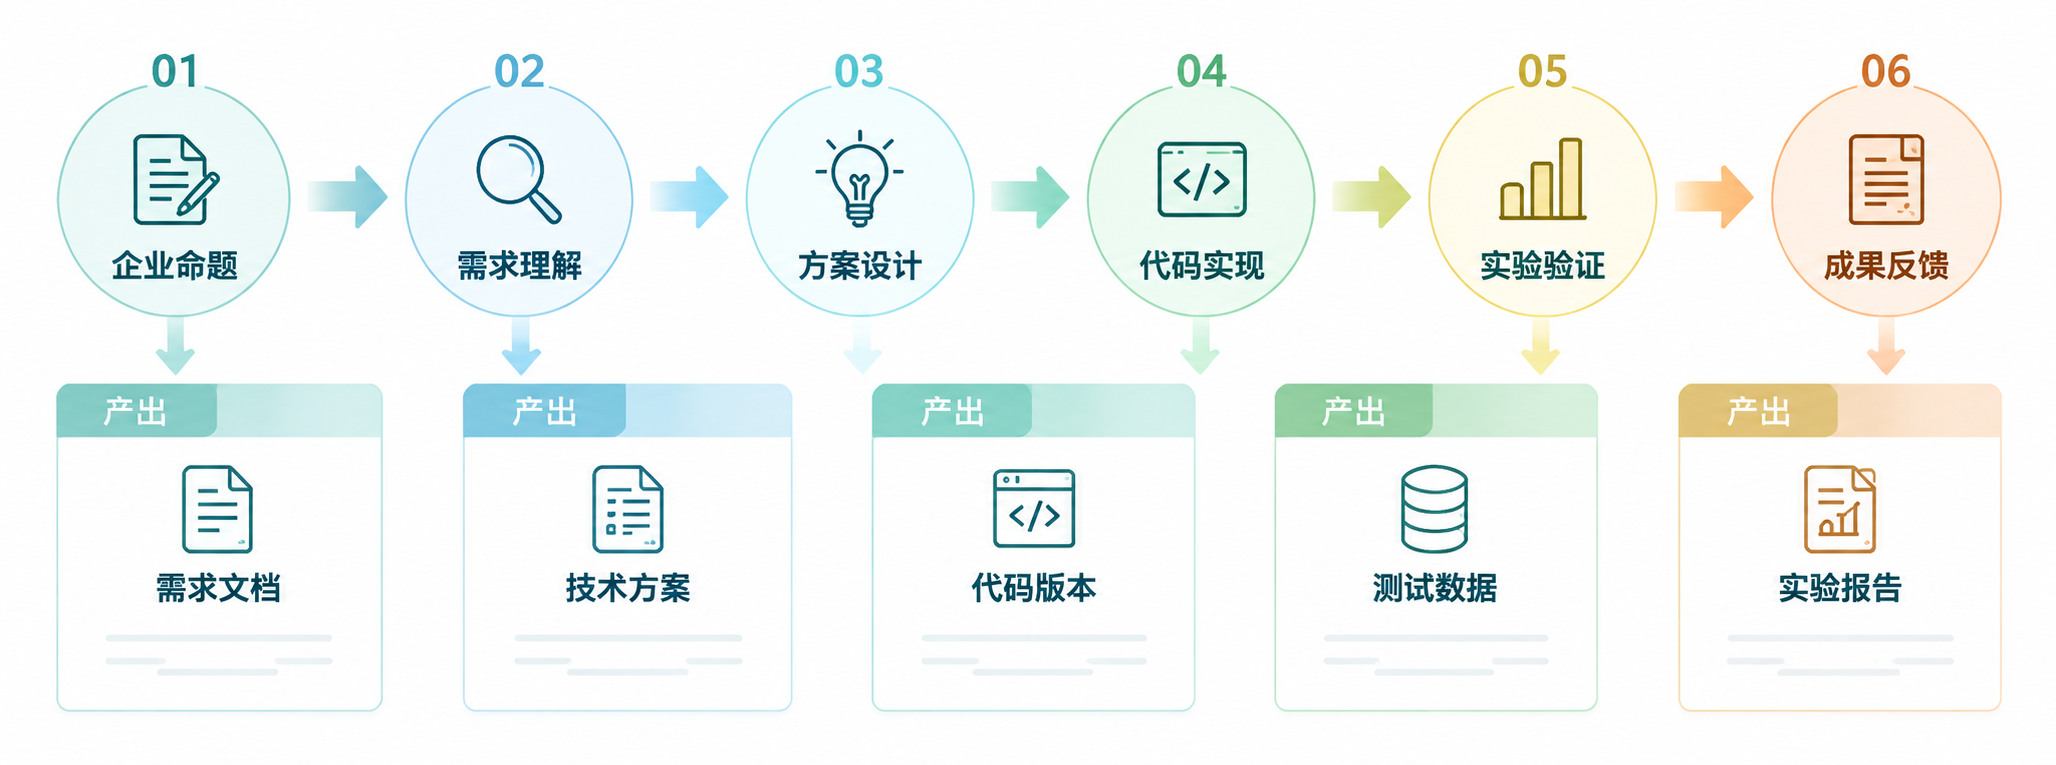
\includegraphics[width=\linewidth,height=.50\textheight,keepaspectratio]{figures/updated-2-1.png}
\caption{项目形成过程与学生参与链条图}\label{fig:2-1}
\end{figure}
\subsection{学生参与机制：需求沟通---培训学习---技术研究---阶段反馈}\label{sec:2.8.2}
学生的持续参与依托一条清晰的链条展开：与企业保持多次沟通和专题会议，围绕命题需求、技术方案和阶段成果持续交流；以 OH 俱乐部为载体开展培训和学习，围绕国产操作系统、智能体运行环境等主题组织专题学习；依托 OH 俱乐部开展技术研究与实验，形成技术报告、测试记录和研究材料；将研究和实验结果整理为阶段成果并向企业反馈，形成下一轮改进的输入。

这一链条保证了学生参与的连续性。与企业的沟通让学生直接面对真实需求的表述方式和验收标准；俱乐部培训把课程中的操作系统、虚拟化、内存管理等知识对接到具体技术栈；技术研究与实验要求学生独立完成方案设计、代码实现和数据复核；阶段反馈则要求学生把技术结果转化为可被企业理解和检验的表述。四个环节相互衔接，避免了“只做实现、不问需求”或“只做汇报、不碰实现”的单点参与。

图 2-2 呈现 OH 俱乐部的运行机制及其在项目中的作用。

\begin{figure}[H]\centering
\setcounter{figure}{1}
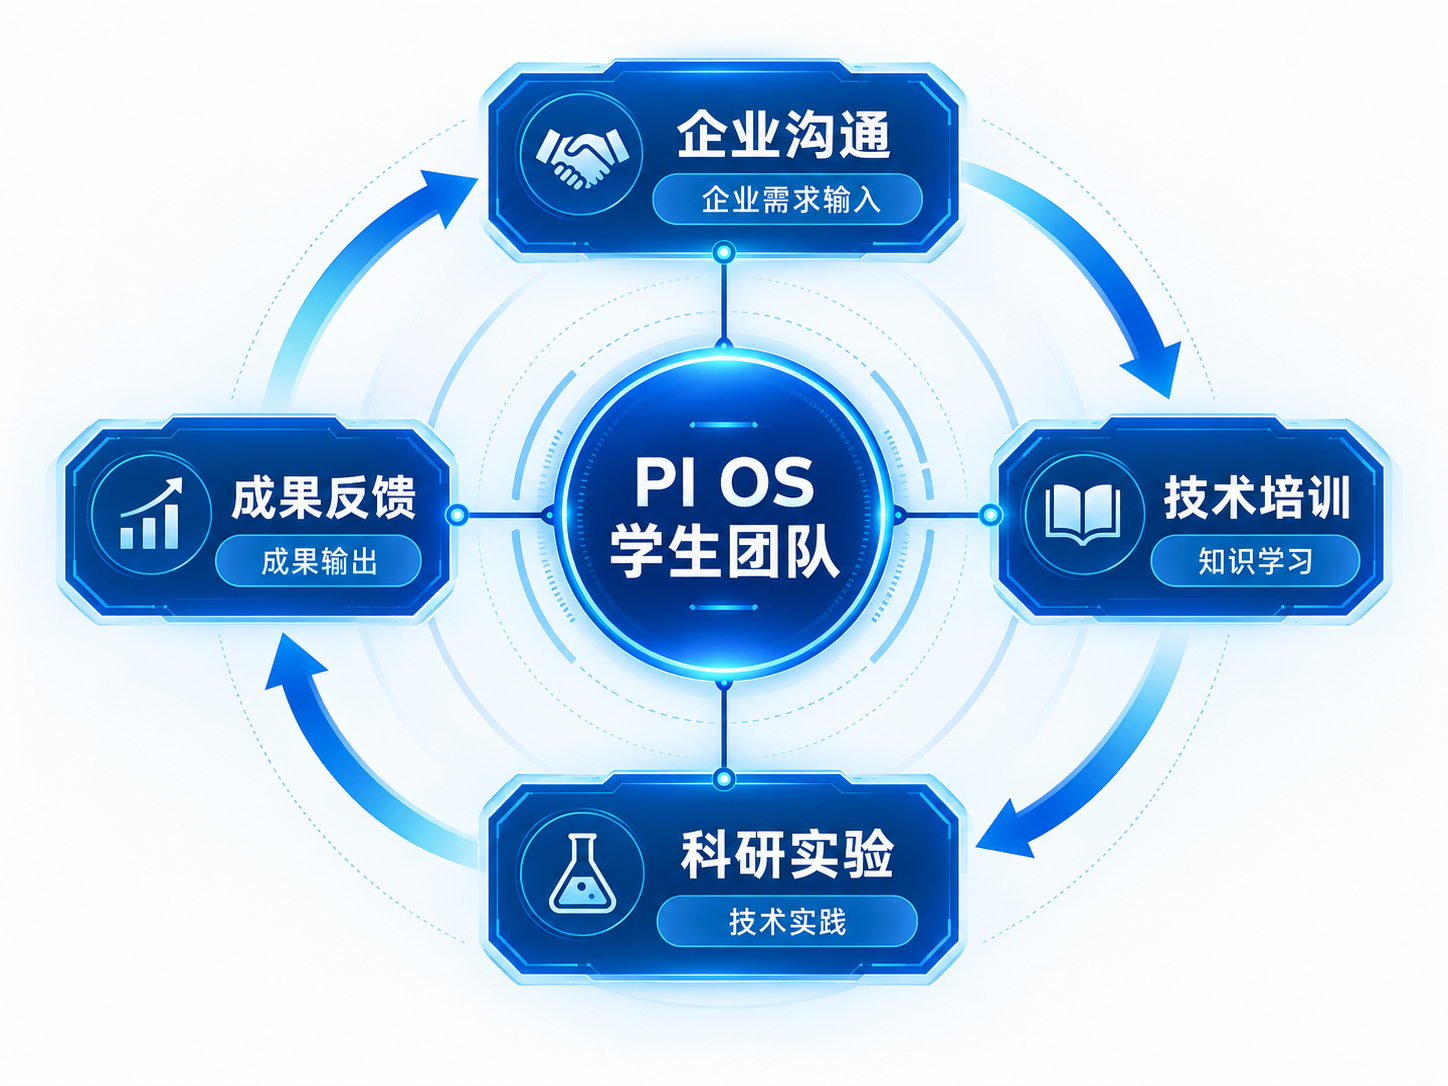
\includegraphics[width=\linewidth,height=.50\textheight,keepaspectratio]{figures/updated-2-2.png}
\caption{OH 俱乐部“培训---研究---反馈”运行机制图}\label{fig:2-2}
\end{figure}
\FloatBarrier
\begingroup\linespread{1}\selectfont
\setcounter{table}{1}
\begin{longtable}{@{}p{\linewidth}@{}}
\caption{OH 俱乐部培训与技术研究活动记录表}\label{tab:2-2}\\
\endfirsthead
\multicolumn{1}{c}{\fontsize{9}{12}\selectfont 表 2-2（续）}\\[4pt]
\endhead
\endfoot\endlastfoot
\begin{minipage}{\linewidth}
\begin{tabular}{@{}>{\raggedright\arraybackslash}p{\dimexpr .21\linewidth-.42\tabcolsep\relax}>{\raggedright\arraybackslash}p{\dimexpr .79\linewidth-1.58\tabcolsep\relax}@{}}
\hline
\rowcolor{WordTableHeader}\multicolumn{2}{@{}p{\linewidth}@{}}{\RecordHeading{编号：T-01\quad 活动主题：命题解读：高密部署智能体沙箱引擎的任务边界与验收口径}} \\ \hline
\rowcolor{white} \TableHeaderText{时间} & 2026 年（待填） \\ \hline
\rowcolor{white} \TableHeaderText{组织与参与} & 组织与主讲：企业技术人员、指导教师\newline 参与学生：全体成员 \\ \hline
\rowcolor{white} \TableHeaderText{形成材料} & 需求理解记录、问题清单（M-01） \\ \hline
\end{tabular}
\end{minipage} \\[6pt]
\begin{minipage}{\linewidth}
\begin{tabular}{@{}>{\raggedright\arraybackslash}p{\dimexpr .21\linewidth-.42\tabcolsep\relax}>{\raggedright\arraybackslash}p{\dimexpr .79\linewidth-1.58\tabcolsep\relax}@{}}
\hline
\rowcolor{WordTableHeader}\multicolumn{2}{@{}p{\linewidth}@{}}{\RecordHeading{编号：T-02\quad 活动主题：openEuler /\allowbreak{} Conch 与 StratoVirt 技术栈入门}} \\ \hline
\rowcolor{white} \TableHeaderText{时间} & 待填 \\ \hline
\rowcolor{white} \TableHeaderText{组织与参与} & 组织与主讲：指导教师、高年级成员\newline 参与学生：全体成员 \\ \hline
\rowcolor{white} \TableHeaderText{形成材料} & 环境搭建指南（ENV-01） \\ \hline
\end{tabular}
\end{minipage} \\[6pt]
\begin{minipage}{\linewidth}
\begin{tabular}{@{}>{\raggedright\arraybackslash}p{\dimexpr .21\linewidth-.42\tabcolsep\relax}>{\raggedright\arraybackslash}p{\dimexpr .79\linewidth-1.58\tabcolsep\relax}@{}}
\hline
\rowcolor{WordTableHeader}\multicolumn{2}{@{}p{\linewidth}@{}}{\RecordHeading{编号：T-03\quad 活动主题：智能体执行流程与工具调用机制：大模型与工具的交替执行}} \\ \hline
\rowcolor{white} \TableHeaderText{时间} & 待填 \\ \hline
\rowcolor{white} \TableHeaderText{组织与参与} & 组织与主讲：刘书雄\newline 参与学生：智能体与卸载机制组 \\ \hline
\rowcolor{white} \TableHeaderText{形成材料} & 流程梳理材料、图 3-1 原始绘制文件 \\ \hline
\end{tabular}
\end{minipage} \\[6pt]
\begin{minipage}{\linewidth}
\begin{tabular}{@{}>{\raggedright\arraybackslash}p{\dimexpr .21\linewidth-.42\tabcolsep\relax}>{\raggedright\arraybackslash}p{\dimexpr .79\linewidth-1.58\tabcolsep\relax}@{}}
\hline
\rowcolor{WordTableHeader}\multicolumn{2}{@{}p{\linewidth}@{}}{\RecordHeading{编号：T-04\quad 活动主题：用户态内核与运行时扁平化设计方法}} \\ \hline
\rowcolor{white} \TableHeaderText{时间} & 待填 \\ \hline
\rowcolor{white} \TableHeaderText{组织与参与} & 组织与主讲：张思淼\newline 参与学生：系统研发组 \\ \hline
\rowcolor{white} \TableHeaderText{形成材料} & 架构说明与组件职责表（V-02） \\ \hline
\end{tabular}
\end{minipage} \\[6pt]
\begin{minipage}{\linewidth}
\begin{tabular}{@{}>{\raggedright\arraybackslash}p{\dimexpr .21\linewidth-.42\tabcolsep\relax}>{\raggedright\arraybackslash}p{\dimexpr .79\linewidth-1.58\tabcolsep\relax}@{}}
\hline
\rowcolor{WordTableHeader}\multicolumn{2}{@{}p{\linewidth}@{}}{\RecordHeading{编号：T-05\quad 活动主题：检查点与恢复机制原理：CRIU、缺页异常与预取}} \\ \hline
\rowcolor{white} \TableHeaderText{时间} & 待填 \\ \hline
\rowcolor{white} \TableHeaderText{组织与参与} & 组织与主讲：陈奕池\newline 参与学生：系统研发组 \\ \hline
\rowcolor{white} \TableHeaderText{形成材料} & 卸载接口说明（S-02） \\ \hline
\end{tabular}
\end{minipage} \\[6pt]
\begin{minipage}{\linewidth}
\begin{tabular}{@{}>{\raggedright\arraybackslash}p{\dimexpr .21\linewidth-.42\tabcolsep\relax}>{\raggedright\arraybackslash}p{\dimexpr .79\linewidth-1.58\tabcolsep\relax}@{}}
\hline
\rowcolor{WordTableHeader}\multicolumn{2}{@{}p{\linewidth}@{}}{\RecordHeading{编号：T-06\quad 活动主题：内存共享机制：引用计数与写时复制}} \\ \hline
\rowcolor{white} \TableHeaderText{时间} & 待填 \\ \hline
\rowcolor{white} \TableHeaderText{组织与参与} & 组织与主讲：刘国威\newline 参与学生：系统研发组 \\ \hline
\rowcolor{white} \TableHeaderText{形成材料} & 共享边界判定规则（S-04） \\ \hline
\end{tabular}
\end{minipage} \\[6pt]
\begin{minipage}{\linewidth}
\begin{tabular}{@{}>{\raggedright\arraybackslash}p{\dimexpr .21\linewidth-.42\tabcolsep\relax}>{\raggedright\arraybackslash}p{\dimexpr .79\linewidth-1.58\tabcolsep\relax}@{}}
\hline
\rowcolor{WordTableHeader}\multicolumn{2}{@{}p{\linewidth}@{}}{\RecordHeading{编号：T-07\quad 活动主题：测试方法与指标口径：基线、重复次数与数据复核}} \\ \hline
\rowcolor{white} \TableHeaderText{时间} & 待填 \\ \hline
\rowcolor{white} \TableHeaderText{组织与参与} & 组织与主讲：李子鹏\newline 参与学生：测试与安全组 \\ \hline
\rowcolor{white} \TableHeaderText{形成材料} & 测试脚本与复核记录（E-01---E-12） \\ \hline
\end{tabular}
\end{minipage} \\[6pt]
\begin{minipage}{\linewidth}
\begin{tabular}{@{}>{\raggedright\arraybackslash}p{\dimexpr .21\linewidth-.42\tabcolsep\relax}>{\raggedright\arraybackslash}p{\dimexpr .79\linewidth-1.58\tabcolsep\relax}@{}}
\hline
\rowcolor{WordTableHeader}\multicolumn{2}{@{}p{\linewidth}@{}}{\RecordHeading{编号：T-08\quad 活动主题：隔离与数据安全：多租户状态共享的安全边界}} \\ \hline
\rowcolor{white} \TableHeaderText{时间} & 待填 \\ \hline
\rowcolor{white} \TableHeaderText{组织与参与} & 组织与主讲：王子硕\newline 参与学生：测试与安全组 \\ \hline
\rowcolor{white} \TableHeaderText{形成材料} & 安全边界说明、表 7-2 相关材料 \\ \hline
\end{tabular}
\end{minipage} \\[6pt]
\end{longtable}\endgroup
\par\noindent{\fontsize{9}{13}\selectfont\linespread{1}\selectfont 注：表中“时间”与“组织与主讲”栏应依据实际活动记录填写，并以签到记录、培训材料或照片等留存；活动编号（T-01---T-08）与表 1-1、表 8-3 中的材料编号一致。尚未开展的活动应补充记录或从本表移除。}

\subsection{学生个人成长记录}\label{sec:2.8.3}
为具体说明学生的成长过程，本节按“承担任务---使用的专业知识---形成的交付物---遇到的问题---能力提升”五个方面，记录部分成员的参与情况。记录内容以实际交付物和测试数据为依据，可在对应材料编号中逐项核对。

\FloatBarrier
\begingroup\linespread{1}\selectfont
\setcounter{table}{2}
\begin{longtable}{@{}p{\linewidth}@{}}
\caption{学生个人成长记录表}\label{tab:2-3}\\
\endfirsthead
\multicolumn{1}{c}{\fontsize{9}{12}\selectfont 表 2-3（续）}\\[4pt]
\endhead
\endfoot\endlastfoot
\begin{minipage}{\linewidth}
\begin{tabular}{@{}>{\raggedright\arraybackslash}p{\dimexpr .21\linewidth-.42\tabcolsep\relax}>{\raggedright\arraybackslash}p{\dimexpr .79\linewidth-1.58\tabcolsep\relax}@{}}
\hline
\rowcolor{WordTableHeader}\multicolumn{2}{@{}p{\linewidth}@{}}{\RecordHeading{姓名与专业：陈奕池\quad 2026 级博士\quad 软件工程}} \\ \hline
\rowcolor{white} \TableHeaderText{承担任务} & 动态资源卸载机制的运行时侧实现，包括状态分类接口、卸载与预取触发路径的代码实现。 \\ \hline
\rowcolor{white} \TableHeaderText{使用的专业知识} & 操作系统内核机制、虚拟化与沙箱运行时、进程状态保存与恢复、内存管理。 \\ \hline
\rowcolor{white} \TableHeaderText{交付成果与材料编号} & 卸载与预加载接口实现（S-02）、struct agent\_park\_task 字段设计说明（V-02）、卸载开销对照测试记录（E-04，对应表 3-1）。 \\ \hline
\rowcolor{white} \TableHeaderText{遇到的问题与能力提升} & 初期按“整体保存”思路实现卸载，实测卸载延迟接近全量快照，说明未抓住状态语义；改为按文件、网络、内存、CPU 和寄存器分类处理、按状态语义分配资源后，卸载开销明显下降。过程中建立了“先量化、再优化”的判断习惯，能够独立完成从机制设计到实验验证的闭环。 \\ \hline
\end{tabular}
\end{minipage} \\[6pt]
\begin{minipage}{\linewidth}
\begin{tabular}{@{}>{\raggedright\arraybackslash}p{\dimexpr .21\linewidth-.42\tabcolsep\relax}>{\raggedright\arraybackslash}p{\dimexpr .79\linewidth-1.58\tabcolsep\relax}@{}}
\hline
\rowcolor{WordTableHeader}\multicolumn{2}{@{}p{\linewidth}@{}}{\RecordHeading{姓名与专业：张思淼\quad 2025 级本科\quad 软件工程}} \\ \hline
\rowcolor{white} \TableHeaderText{承担任务} & 运行时扁平化方案的设计与说明，梳理 LibOS、Services、Std 接口、Visor、Sched/\allowbreak{}Proxyd/\allowbreak{}Orchest 的职责边界。 \\ \hline
\rowcolor{white} \TableHeaderText{使用的专业知识} & 操作系统结构、网络协议栈、文件系统、系统架构设计。 \\ \hline
\rowcolor{white} \TableHeaderText{交付成果与材料编号} & 扁平化架构说明与组件职责表（V-02）、图 3-4 架构图原始文件、单实例内存构成测量记录（E-02，对应图 3-3）。 \\ \hline
\rowcolor{white} \TableHeaderText{遇到的问题与能力提升} & 最初把“扁平化”理解为简单合并组件，无法解释固定开销为何随实例数增长；通过逐项测量 Runtime、Sandbox 与 Waste 的内存构成，学会用可测指标界定设计目标，架构表达能力明显提升。 \\ \hline
\end{tabular}
\end{minipage} \\[6pt]
\begin{minipage}{\linewidth}
\begin{tabular}{@{}>{\raggedright\arraybackslash}p{\dimexpr .21\linewidth-.42\tabcolsep\relax}>{\raggedright\arraybackslash}p{\dimexpr .79\linewidth-1.58\tabcolsep\relax}@{}}
\hline
\rowcolor{WordTableHeader}\multicolumn{2}{@{}p{\linewidth}@{}}{\RecordHeading{姓名与专业：刘书雄\quad 2024 级本科\quad 人工智能}} \\ \hline
\rowcolor{white} \TableHeaderText{承担任务} & 智能体任务流程梳理、动态卸载与预取机制说明。 \\ \hline
\rowcolor{white} \TableHeaderText{使用的专业知识} & 智能体执行框架、工具调用协议、大模型推理流程、Python 运行时。 \\ \hline
\rowcolor{white} \TableHeaderText{交付成果与材料编号} & 大模型与工具交替调用流程分析（图 3-1 原始材料）、六类典型 Agent 负载资源画像（图 3-2、E-03）、语义感知实现路径说明（第 3.5.3 节）。 \\ \hline
\rowcolor{white} \TableHeaderText{遇到的问题与能力提升} & 起初以“任务整体耗时”描述性能，无法说明资源在何时被浪费；改为按 init、step 等阶段对齐 CPU 与内存时序后，能够定位等待阶段的内存驻留窗口（CPU 峰值 209.7\%，内存维持约 447.7MB）。由此掌握了以时序数据支撑机制设计的方法。 \\ \hline
\end{tabular}
\end{minipage} \\[6pt]
\begin{minipage}{\linewidth}
\begin{tabular}{@{}>{\raggedright\arraybackslash}p{\dimexpr .21\linewidth-.42\tabcolsep\relax}>{\raggedright\arraybackslash}p{\dimexpr .79\linewidth-1.58\tabcolsep\relax}@{}}
\hline
\rowcolor{WordTableHeader}\multicolumn{2}{@{}p{\linewidth}@{}}{\RecordHeading{姓名与专业：李子鹏\quad 2025 级本科\quad 计算机科学与技术}} \\ \hline
\rowcolor{white} \TableHeaderText{承担任务} & 测试数据复核、指标计算、测试环境与验收材料整理。 \\ \hline
\rowcolor{white} \TableHeaderText{使用的专业知识} & 性能测试方法、统计分析、Linux 资源监控、数据可视化。 \\ \hline
\rowcolor{white} \TableHeaderText{交付成果与材料编号} & 测试脚本（S-01---S-06）、受限资源下系统级对照测试数据（E-06，对应表 3-2）、48 个任务并发测试记录（E-01）。 \\ \hline
\rowcolor{white} \TableHeaderText{遇到的问题与能力提升} & 首轮测试未固定任务数、重复次数与错峰拉起间隔，两次结果差异较大且无法归因；建立“基线---变量---重复次数---口径”统一模板并采用 5 次取中位数后，数据可复核性明显提高。认识到测试条件本身就是结论的一部分。 \\ \hline
\end{tabular}
\end{minipage} \\[6pt]
\begin{minipage}{\linewidth}
\begin{tabular}{@{}>{\raggedright\arraybackslash}p{\dimexpr .21\linewidth-.42\tabcolsep\relax}>{\raggedright\arraybackslash}p{\dimexpr .79\linewidth-1.58\tabcolsep\relax}@{}}
\hline
\rowcolor{WordTableHeader}\multicolumn{2}{@{}p{\linewidth}@{}}{\RecordHeading{姓名与专业：周以恒\quad 2026 级硕士\quad 计算机科学与技术}} \\ \hline
\rowcolor{white} \TableHeaderText{承担任务} & 系统研究、技术文档审核与方案复核支持，负责技术指标口径统一。 \\ \hline
\rowcolor{white} \TableHeaderText{使用的专业知识} & 计算机系统结构、实验设计与可复现性方法、技术写作。 \\ \hline
\rowcolor{white} \TableHeaderText{交付成果与材料编号} & 技术文档审核记录与修改意见（V-03）、指标口径与证据编号规则（M-04）、团队协作与质量控制机制（表 8-2）。 \\ \hline
\rowcolor{white} \TableHeaderText{遇到的问题与能力提升} & 审阅中发现同一指标在不同材料中存在“目标值”与“实测值”混用的情况，容易被理解为结果倒退；据此建立“已实测 /\allowbreak{} 阶段结果 /\allowbreak{} 目标值 /\allowbreak{} 待验收”四类状态标签并推广到全部技术材料。跨模块一致性校验能力得到提升。 \\ \hline
\end{tabular}
\end{minipage} \\[6pt]
\end{longtable}\endgroup
\par\noindent{\fontsize{9}{13}\selectfont\linespread{1}\selectfont 注：表中成员专业与职责与表 8-1 保持一致；交付物编号与表 8-3 成员贡献矩阵对应，原始材料由项目组统一归档保存，可按编号调阅。}

图 2-3 以能力维度汇总成员在项目中的成长分布。

\begin{figure}[H]\centering
\setcounter{figure}{2}
\begin{tikzpicture}[x=1cm,y=1cm, every node/.style={font=\fontsize{9}{12}\selectfont\linespread{1}\selectfont,align=center},box/.style={draw=DiagramRule,rounded corners=2pt,fill=DiagramLight,inner sep=6pt},arr/.style={->,>=stealth,thick,draw=DiagramMain}]
\node[box,text width=12cm,] (h) at (6,0) {\textbf{成员任务与能力维度对应}\quad 依据表 2-3，仅标示有具体交付物支撑的主要任务};
\node[box,text width=1.9cm,fill=DiagramMain,text=white] (c0) at (2.7,-1.2) {系统与内核};
\node[box,text width=1.9cm,fill=DiagramMain,text=white] (c1) at (4.95,-1.2) {实验与复核};
\node[box,text width=1.9cm,fill=DiagramMain,text=white] (c2) at (7.2,-1.2) {智能体机制};
\node[box,text width=1.9cm,fill=DiagramMain,text=white] (c3) at (9.45,-1.2) {文档与复现};
\node[box,text width=1.9cm,fill=DiagramMain,text=white] (c4) at (11.7,-1.2) {协作与统筹};
\node[box,text width=1.1cm,] (n0) at (0.45,-2.2) {陈奕池};
\node[box,text width=1.9cm,minimum height=.7cm,fill=DiagramMedium] (m00) at (2.7,-2.2) {S-02 /\allowbreak{} V-02};
\node[box,text width=1.9cm,minimum height=.7cm,fill=DiagramMedium] (m01) at (4.95,-2.2) {E-04};
\node[box,text width=1.9cm,minimum height=.7cm,fill=white] (m02) at (7.2,-2.2) {---};
\node[box,text width=1.9cm,minimum height=.7cm,fill=white] (m03) at (9.45,-2.2) {---};
\node[box,text width=1.9cm,minimum height=.7cm,fill=white] (m04) at (11.7,-2.2) {---};
\node[box,text width=1.1cm,] (n1) at (0.45,-3.1) {张思淼};
\node[box,text width=1.9cm,minimum height=.7cm,fill=DiagramMedium] (m10) at (2.7,-3.1) {V-02};
\node[box,text width=1.9cm,minimum height=.7cm,fill=DiagramMedium] (m11) at (4.95,-3.1) {E-02};
\node[box,text width=1.9cm,minimum height=.7cm,fill=white] (m12) at (7.2,-3.1) {---};
\node[box,text width=1.9cm,minimum height=.7cm,fill=DiagramMedium] (m13) at (9.45,-3.1) {图 3-4};
\node[box,text width=1.9cm,minimum height=.7cm,fill=white] (m14) at (11.7,-3.1) {---};
\node[box,text width=1.1cm,] (n2) at (0.45,-4.0) {刘书雄};
\node[box,text width=1.9cm,minimum height=.7cm,fill=white] (m20) at (2.7,-4.0) {---};
\node[box,text width=1.9cm,minimum height=.7cm,fill=white] (m21) at (4.95,-4.0) {---};
\node[box,text width=1.9cm,minimum height=.7cm,fill=DiagramMedium] (m22) at (7.2,-4.0) {E-03};
\node[box,text width=1.9cm,minimum height=.7cm,fill=DiagramMedium] (m23) at (9.45,-4.0) {图 3-1 /\allowbreak{} 3-2};
\node[box,text width=1.9cm,minimum height=.7cm,fill=white] (m24) at (11.7,-4.0) {---};
\node[box,text width=1.1cm,] (n3) at (0.45,-4.9) {李子鹏};
\node[box,text width=1.9cm,minimum height=.7cm,fill=white] (m30) at (2.7,-4.9) {---};
\node[box,text width=1.9cm,minimum height=.7cm,fill=DiagramMedium] (m31) at (4.95,-4.9) {E-01 /\allowbreak{} E-06};
\node[box,text width=1.9cm,minimum height=.7cm,fill=white] (m32) at (7.2,-4.9) {---};
\node[box,text width=1.9cm,minimum height=.7cm,fill=DiagramMedium] (m33) at (9.45,-4.9) {S-01---S-06};
\node[box,text width=1.9cm,minimum height=.7cm,fill=white] (m34) at (11.7,-4.9) {---};
\node[box,text width=1.1cm,] (n4) at (0.45,-5.800000000000001) {周以恒};
\node[box,text width=1.9cm,minimum height=.7cm,fill=white] (m40) at (2.7,-5.800000000000001) {---};
\node[box,text width=1.9cm,minimum height=.7cm,fill=white] (m41) at (4.95,-5.800000000000001) {---};
\node[box,text width=1.9cm,minimum height=.7cm,fill=white] (m42) at (7.2,-5.800000000000001) {---};
\node[box,text width=1.9cm,minimum height=.7cm,fill=DiagramMedium] (m43) at (9.45,-5.800000000000001) {V-03 /\allowbreak{} M-04};
\node[box,text width=1.9cm,minimum height=.7cm,fill=DiagramMedium] (m44) at (11.7,-5.800000000000001) {表 8-2};
\node[box,text width=12cm,] (note) at (6,-7.15) {注：空白表示本表未列出对应交付物，不代表成员不具备该项能力。};
\end{tikzpicture}
\caption{学生能力成长矩阵图}\label{fig:2-3}
\end{figure}
\subsection{学生成长的过程性证据与编号规则}\label{sec:2.8.4}
为使“学生成长”可被核对，而不停留在描述层面，项目对过程材料采用统一编号规则，并在正文中直接引用编号。编号规则如下：

\begingroup\linespread{1}\fontsize{10.5pt}{14pt}\selectfont
\NumberedPara{1}{M-xx：与企业沟通形成的会议纪要、需求确认记录与阶段反馈记录，记载时间、参与人、议题与结论；}
\NumberedPara{2}{T-xx：OH 俱乐部培训与专题学习记录，记载主题、主讲、参与学生与形成材料；}
\NumberedPara{3}{E-xx：实验与测试记录，包含环境、负载、任务数、重复次数与原始数据；}
\NumberedPara{4}{S-xx：实验脚本与可复现说明，保证同一实验可由其他成员独立复现；}
\NumberedPara{5}{ENV-xx：测试环境配置记录，包括硬件规格、镜像版本、参数设置以及关闭 Swap 等约束条件；}
\NumberedPara{6}{V-xx：代码与文档版本记录，标记每次关键修改的责任人与复核人；}
\NumberedPara{7}{I-xx：一手调研访谈与需求确认记录，记载受访角色、时间、方式与结论。}
\par\endgroup
\clearpage
\FloatBarrier
\begingroup\linespread{1}\selectfont
\setcounter{table}{3}
\begin{longtable}{@{}>{\raggedright\arraybackslash}p{\dimexpr 0.14106\linewidth-1.1285\tabcolsep\relax}>{\raggedright\arraybackslash}p{\dimexpr 0.26042\linewidth-2.0833\tabcolsep\relax}>{\raggedright\arraybackslash}p{\dimexpr 0.13563\linewidth-1.0851\tabcolsep\relax}>{\raggedright\arraybackslash}p{\dimexpr 0.17361\linewidth-1.3889\tabcolsep\relax}>{\raggedright\arraybackslash}p{\dimexpr 0.28928\linewidth-2.3142\tabcolsep\relax}@{}}
\caption{学生参与过程证据清单}\label{tab:2-4}\\
\hline
\rowcolor{WordTableHeader} \TableHeaderText{编号} & \TableHeaderText{材料名称} & \TableHeaderText{形成时间} & \TableHeaderText{主要形成人} & \TableHeaderText{可支撑的结论} \\ \hline
\endfirsthead
\multicolumn{5}{c}{\fontsize{9}{12}\selectfont 表 2-4（续）}\\
\hline
\rowcolor{WordTableHeader} \TableHeaderText{编号} & \TableHeaderText{材料名称} & \TableHeaderText{形成时间} & \TableHeaderText{主要形成人} & \TableHeaderText{可支撑的结论} \\ \hline
\endhead
\hline\endfoot\hline\endlastfoot
\rowcolor{WordTableStripe} 
M-01 & 命题解读与需求确认纪要 & 2026 年（待填） & 张纪同、刘书雄 & 学生直接参与需求理解，明确 16GB 总内存、2U8G 可见规格、关闭 Swap 等验收约束 \\ \hline
M-02 & 技术方案专题讨论纪要 & 待填 & 陈奕池、张思淼 & 三项技术问题的划分依据与方案选择过程 \\ \hline
\rowcolor{WordTableStripe} 
M-03 & 阶段成果反馈纪要 & 待填 & 张纪同、周以恒 & 阶段结果向企业反馈并形成下一轮改进输入 \\ \hline
T-01---T-08 & OH 俱乐部培训与技术研究活动记录 & 待填 & 各主题主讲人 & 学生在国产操作系统与智能体运行环境方向形成系统学习记录 \\ \hline
\rowcolor{WordTableStripe} 
E-01---E-12 & 实验与测试日志 & 待填 & 李子鹏及各模块主责人 & 关键指标可复核，均标注环境、任务数与重复次数 \\ \hline
S-01---S-06 & 实验脚本与复现说明 & 待填 & 李子鹏、陈奕池 & 实验结果可由其他成员独立复现 \\ \hline
\rowcolor{WordTableStripe} 
ENV-01---ENV-03 & 测试环境配置记录 & 待填 & 李子鹏 & 研究环境与华为指定环境的测试条件明确区分 \\ \hline
V-01---V-05 & 代码与文档版本记录 & 待填 & 各模块主责人、周以恒 & 关键修改均有责任人、复核人与时间记录 \\ \hline
\end{longtable}\endgroup
\par\noindent{\fontsize{9}{13}\selectfont\linespread{1}\selectfont 注：表中标注“待填”的时间与责任人应按实际记录补齐后再提交；未形成记录的活动应补充记录或从本表移除，避免材料与描述不一致。项目每完成一轮推进，应同步更新本表。}

图 2-4 呈现过程材料的编号体系与流转关系。

\begin{figure}[H]\centering
\setcounter{figure}{3}
\begin{tikzpicture}[x=1cm,y=1cm,every node/.style={font=\fontsize{9}{11}\selectfont\linespread{1}\selectfont,align=center},box/.style={draw=DiagramRule,rounded corners=2pt,fill=DiagramLight,inner sep=3pt},arr/.style={->,>=stealth,draw=DiagramMain}]
\node[box,text width=2.85cm] (a) at (1.65,0) {\textbf{企业沟通}\\M-xx\\会议与需求记录};
\node[box,text width=2.85cm] (b) at (4.9,0) {\textbf{培训学习}\\T-xx\\培训与专题学习};
\node[box,text width=2.85cm] (c) at (8.15,0) {\textbf{实验测试}\\E-xx\\实验与测试日志};
\node[box,text width=2.85cm] (d) at (11.4,0) {\textbf{需求调研}\\I-xx\\调研与需求确认};
\node[box,text width=12.4cm] (support) at (6.5,-1.25) {\textbf{配套材料}：S-xx 脚本与复现说明\quad ENV-xx 测试环境配置\quad V-xx 代码与文档版本};
\draw[arr] (a.south) -- (support.north -| a.south);
\draw[arr] (b.south) -- (support.north -| b.south);
\draw[arr] (c.south) -- (support.north -| c.south);
\draw[arr] (d.south) -- (support.north -| d.south);
\node[box,text width=12.4cm,fill=DiagramMain,text=white] (archive) at (6.5,-2.25) {责任人提交 → 复核人确认 → 统一归档 → 正文按编号引用与调阅};
\draw[arr] (support) -- (archive);
\node[box,text width=12.4cm] (note) at (6.5,-3.2) {实验数据同时关联环境配置与复现脚本；编号区间与记录状态见表 2-4。};
\end{tikzpicture}
\caption{学生成长过程证据编号与流转关系图}\label{fig:2-4}
\end{figure}
